\documentclass{beamer}
\usepackage{graphicx}
\usepackage{tikz}
\usetikzlibrary{shapes,arrows}
\usepackage{tikz}
\usetheme{default}
%\usecolortheme{seahorse}
\usepackage{default}
  \setbeamertemplate{footline}[page number]

\setbeamertemplate{navigation symbols}{}
\setbeamertemplate{frametitle}[default][center]
\setbeamerfont{frametitle}{shape=\scshape}

\usepackage{xcolor}

\usepackage[flushleft]{threeparttable}

{\title{\textsc{Numerical Methods-Lecture XIII: \\ Dynamic Discrete Choice Estimation} \\ \tiny (See Rust 1987)}
\date{}
\author{Trevor Gallen}

\begin{document}
\renewcommand*{\inserttotalframenumber}{\pageref{lastframe}}

\begin{frame}
\titlepage
\end{frame}


\section{Introduction}
\subsection{Introduction}
\begin{frame}
\frametitle{Introduction}
\begin{itemize}
\item Rust (1987) wrote a paper about Harold Zurcher's decisions as the superintendent 
of maintenance at the Madison (Wisconsin) Metropolitan Bus Company. 
\bigskip
\begin{itemize}
\item 10 years of monthly data 
\bigskip
\item bus mileage and engine replacement
\bigskip
\item 104 buses
\bigskip
\item 1 Harold
\bigskip
\end{itemize} 
\item<2-> Not interested in Harold per se
\bigskip
\item<3-> Interested in application of Dynamic Discrete Choice framework
\bigskip
\end{itemize}
\end{frame}


\begin{frame}
\frametitle{Description}
\begin{itemize}
\item Observe monthly bus mileage
\bigskip
\item Observe maintenance diary with date, milage, and list of components repaired or replaced
\bigskip
\item Three types of maintenance operations
\begin{itemize}
\item Routine adjustments (brake adjustments, tire rotation)
\bigskip
\item Replacement of individual components when failed
\bigskip
\item \color<2->{red}{Major engine overhauls}
\bigskip
\end{itemize}
\item Model Zurcher's decision to replace bus engines based on observables \emph{and unobservables}
\end{itemize}
\end{frame}

\begin{frame}
\frametitle{Model }
\begin{itemize}
\item Agent is forward looking
\bigskip
\item Maximizes expected intertemporal payoff
\bigskip
\item Estimate parameters of the models 
\bigskip
\item Test whether the agent's behavior is consistent with the model
\end{itemize}
\end{frame}


\begin{frame}
\frametitle{Replacement data-I}
\begin{center}
\begin{figure}[h!]
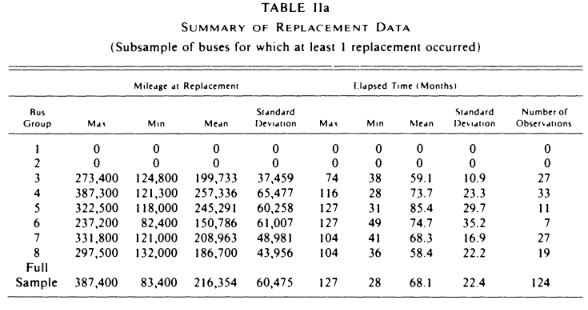
\includegraphics[scale =0.5]{replacement_data1.png}
\end{figure}
\end{center}
\end{frame}

\begin{frame}
\frametitle{Replacement data-II}
\begin{center}
\begin{figure}[h!]
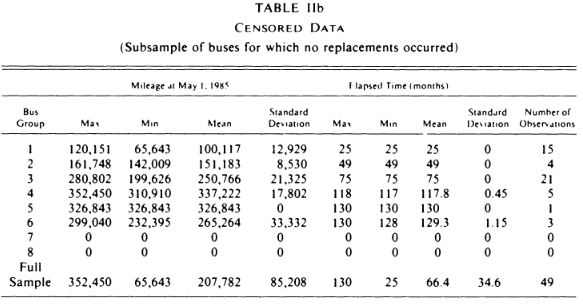
\includegraphics[scale =0.5]{replacement_data2.png}
\end{figure}
\end{center}
\end{frame}


\begin{frame}
\frametitle{Replacement data-III}
\begin{center}
\begin{figure}[h!]
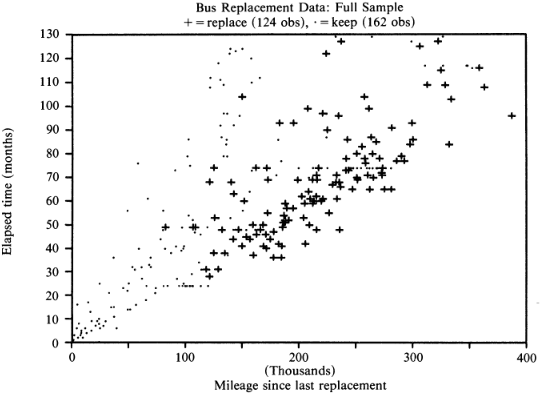
\includegraphics[scale =0.5]{replacement_data.png}
\end{figure}
\end{center}
\end{frame}

\begin{frame}
\frametitle{Sample }
\begin{itemize}
\item Focus on bus groups 1-4
\bigskip
\item Most recent acquisitions
\bigskip
\item Have data on replacement costs only for this group
\bigskip
\item Utilization fairly constant within each group (necessary for model)
\end{itemize}
\end{frame}

\begin{frame}
\frametitle{Model - I}
\begin{itemize}
\item Harold chooses $\{i_1,i_2,{...},i_t,{...}\}$ to maximize his expected utility
\end{itemize}
\[ \max_{\{i_1,i_2,{...},i_t,{...}\}}E_t\sum_{t=1}^\infty \beta^{t-1} u(x_t,\varepsilon_t,i_t;\theta)\]
\begin{itemize}
\item  $x_t$ is the total mileage on an engine since last replacement
\bigskip
\item $\varepsilon_t$ are unobservable (to the econometrician) shocks
\bigskip
\item $i_t$ is an indicator of engine replacement
\bigskip
\item $\theta$ is vector of parameters (to be discussed below)
\end{itemize}

\end{frame}


\begin{frame}
\frametitle{Model - II}
\begin{itemize}
\item Cost function 
\end{itemize}
\[ c(x,\theta_1)=m(x,\theta_{11}) +\mu(x,\theta_{12})b(x,\theta_{13})\]
\begin{itemize}
\item $m(x,\theta_{11})$ is the conditional expectation of normal maintenance and operation expenditure
\bigskip
\item $\mu(x,\theta_{12})$ is the conditional probability of an unexpected engine failure
\bigskip
\item $b(x,\theta_{13})$ is the conditional expectation of towing costs, repair costs, and loss of customer goodwill costs resulting from engine failure
\bigskip
\item No data on maintenance and operating costs, so only estimating the sum of costs $c(x,\theta_1)$ 
\end{itemize}
\end{frame}



\begin{frame}
\frametitle{Model - III}
\begin{itemize}
\item Stochastic process governing $\{i_t,x_t\}$ is the solution to 
\end{itemize}
\[ V_\theta(x_t) = \sup_{\Pi} E\left\{\sum_{j=t}^\infty \beta^{j-t}u(x_j,f_j,\theta_1)\left| x_t\right.\right\}\]
\begin{itemize}
\item where utility $u$ is given by 
\end{itemize}
\[ u(x_t,i_t,\theta_1) = \left\{ \begin{array}{ccc} -c(x_t,\theta_1) & if &i_t=0\\
-\left[ \ \overline{P} - \underline{P} + c(0,\theta_1)\right]& if & i_t = 1\end{array}\right.  \]
\begin{itemize}
\item $\Pi=\{f_t,f_{t+1},{...}\}$ is a sequence of decision rules where 
\bigskip
\item each $f$ indicates the optimal choice (replace or not) at time $t$ given the entire history of investment $i_{t-1},...,i_1$ and mileage $x_t,x_{t-1},...,x_1$ observed to date
\bigskip
\item $\underline{P}$ is the scrap value of an engine
\bigskip
\item $\overline{P}$ is the cost of a new engine
\end{itemize}
\end{frame}


\begin{frame}
\frametitle{Model - IV}
\begin{itemize}
\item  Evolution of $x_t$ is given by stochastic process: 
\end{itemize}
$p(x_{t+1}|x_t,i_t,\theta_2)$
\[=\left\{\begin{array}{lcccc} \theta_2 \exp[\theta_2(x_{t+1}-x_t)] & if & i_t=0& \&& x_{t+1}\geq x_t\\
\theta_2 \exp[\theta_2(x_{t+1})]& if & i_t=1&\&&x_{t+1}\geq0\\
0 &o/w&&&  \end{array}\right.\]
\begin{itemize}
\item Without investment, next period mileage is drawn from exponential CDF $1-\exp[\theta_2(x_{t+1}-x_{t})]$  
\bigskip
\item With investment, next period mileage is drawn from exponential CDF $1-\exp[\theta_2(x_{t+1}-0)]$  
\end{itemize}
\end{frame}

\begin{frame}
\frametitle{Model - V}
 Bellman:
\[V_{\theta}(x_t)=\max_{i_t\in \{0,1\}}u(x_t,i_t,\theta_1)+\beta EV_{\theta}(x_t,i_t)\]

\[EV_{\theta}(x_t,i_t)=\int_o^\infty V_{\theta}(y)P(dy|x_t,i_t,\theta_2)\]
\[i_t=f(x_t,\theta)=\left\{\begin{array}{lcc}1 & if & x_t>\gamma(\theta_1,\theta_2)\\ 0 & if&x_t\leq \gamma(\theta_1,\theta_2)\end{array}\right.\]
\begin{itemize}
\item Where $\gamma(\theta_1,\theta_2)$ is the investment cut-off (``optimal stopping barrier") given by the unique solution to 
\end{itemize}
\[ ( \ \overline{P} - \underline{P})(1-\beta)=\int_0^{\gamma(\theta_1,\theta_2)}[1-\beta\exp\{-\theta_2(1-\beta)y\}]\frac{\partial c(y,\theta_1)}{\partial y dy}\]
\textcolor{red}{We have a closed-form solution!?}
 \end{frame}


\begin{frame}
\frametitle{Model - VI}
\begin{itemize}
\item Problem:  all engines are replaced at same point.
\bigskip
\item How do we solve this? (In standard MLE)?
\bigskip
\item<2-> Add an error term:
$$i_t=f(x_t,\theta)+\varepsilon_t$$
\item<3-> But that's dumb!  Why?
\bigskip
\item<4-> Whoops!  Accidentally replaced! (Assuming agent is making decisions without thinking about the error term before this period)
\bigskip
\item<4-> Reinterpret: $\varepsilon_t$ is an unobservable state variable known to the agent but not the econometrician
\bigskip
\item<5-> \textcolor{red}{Add structure so model is consistent: no ``mistakes" just unobserved to econometrician but not agent data}
\end{itemize}
\end{frame}

\begin{frame}
\frametitle{Model - VII}
\small
\begin{tabular}{l|p{7cm}|}
$C(x_t)$ &Choice set. A finite set of allowable values of the control variable $i_t$ when state variable is $x_t$\\
$\varepsilon_t=\{e_t(i)|i\in C(x_t)\}$&A $\# C(x_t)$-dimensional vector of state variables observed by agent by not by the econometrician. \\
$x_t=\{x_t(1),{...},x_t(K)\}$&$K-$dimensional vector of state variables observed by both the agent and the econometrician.\\
$u(x_t,i_t,\theta_1)+\varepsilon_t(i)$&Realized single period utility of decision $i$ when state variable is $x_t,\varepsilon_t)$. $\theta_1$ is a vector of unknown parameters to be estimated\\
$p(x_{t+1},\varepsilon_{t+1}|x_t,\varepsilon_t,i_t,\theta_2,\theta_3)$&\text{Markov transitional denisty for state variable } $(x_t,\varepsilon_t)$ when alternative $i_t$ is selected. $\theta_1$ and $\theta_2$ are vectors of unknown parameters to be estimated.\\
$\theta=(\beta,\theta_1,\theta_2,\theta_3)$&The complete $1+K_1+K_2+K_3$ vector of parameters to be estimated
\end{tabular} 

\end{frame}



\begin{frame}
\frametitle{Model - VIII}
Now we have our dynamic discrete choice model.  Infinite horizon, discounted Harold decision problem:
\[V_\theta(x_t,\varepsilon_t)=\sup_{\Pi}E\left\{\left.\sum_{j=t}^\infty \beta^{j-t}\left(u(x_j,f_j,\theta_1)+\varepsilon_j(f_j)\right)\right|x_t,\varepsilon_t,\theta_2,\theta_3\right\}\] The optimal value function $V_\theta$ is the unique solution to \[V_\theta(x_t,\varepsilon_t)=\max_{i_t\in C(x_t)}[u(x_t,i_t,\theta_1)+\varepsilon_t(i)+\beta EV_\theta(x_t,\varepsilon_t,i_t)] \] with the decision rule \[i_t=f(x_t,\varepsilon_t,\theta)\equiv arg\max_{i_t\in C(x_t)}[u(x_t,i_t,\theta_1)+\varepsilon_t(i_t)+\beta EV_\theta(x_t,\varepsilon_t,i_t)]\]

\end{frame}

\begin{frame}
\frametitle{Model - IX}
Problems:
\begin{itemize}
\item $\varepsilon_t$ appears nonlinearly. Have to integrate out over $\varepsilon_t$ to obtain choice probabilities
\bigskip
\item  Dimensionality: grid approach to estimating $\varepsilon$ would still be too large to be computationally tractable (especially in 1987). 
\end{itemize}

\end{frame}

\begin{frame}
\frametitle{Model - X}
\begin{itemize}
\item Don't want to integrate over all possible $x_t$ and $\epsilon_t$ combinations
\bigskip
\item Fortunately, this problem is separable (the two are unrelated):
\bigskip
\item Conditional Independence Assumption:
\[P(x_{t+1},\varepsilon_{t+1}|x_t,\varepsilon_t,i,\theta_2,\theta_3)=\textcolor{blue}{q(\varepsilon_{t+1}|x_{t+1},\theta_2)}\textcolor{red}{P(x_{t+1}|x_t,i,\theta_3)}\]
\bigskip
\item \textcolor{red}{Estimate the transition matrix of miles}
\bigskip
\item \textcolor{blue}{Then, given the miles today, have disturbance term}
\end{itemize}
%Gives us two theorems [ADD]
\end{frame}


\begin{frame}
\frametitle{Estimation-I}
\begin{itemize}
\item Three likelihood functions. Two partial likelihoods, and one full.
\bigskip
\item Mileage transition probability (first step)
\[ \ell^1(x_1,{...},x_T,i_1,{...},i_T|x_0,i_0,\theta)=\prod_{t=1}^Tp(x_t|x_{t-1},i_{t-1},\theta_3)\]
\item Choice given mileage (and shock) (second step)
\[\ell^2(x_1,{...},x_{T},i_1,{...},i_T|\theta)=\prod_{t=1}^TP(i_t|x_t,\theta)\]
And the full likelihood function:
\[\ell^f(x_1,{...},x_T,i_1,{...},i_T|x_0,i_0,\theta)=\prod_{t=1}^TP(i_t|x_t,\theta)p(x_t|x_{t-1},i_{t-1},\theta_3)\]
Three stages of estimation.
\end{itemize}
\end{frame}

\begin{frame}
\frametitle{Estimation-II}
Recall, have value function which is given by the functional equation  \[EV_\theta(x,i)=\int_y\log\left\{ \sum_{j\in C(y)}\exp(u(y,j,\theta_1)+\beta EV_\theta (y,j))\right\}p(dy|x,i,\theta_3)\]
Goal is to estimate $\theta$ using a nested fixed point algorithm:
\begin{itemize}
\item For each $\theta$, compute $EV_\theta$ using a fixed point algorithm
\bigskip 
\item Outer hill climbing algorithm searches for the value of $\theta$ which maximizes the likelihood function.
\end{itemize}
\end{frame}

\begin{frame}
\frametitle{Estimation-III}
First estimate the parameters $\theta_3$ of the transition probability \[p(x_{t+1}|x_t,i_t,\theta_3)=\left\{\begin{array}{lll}g(x_{t+1}-x_t,\theta_3)&if&i_t=1\\ g(x_{t+1}-0,\theta_3)&if&i_t=0\end{array}\right.\]
Using\[ \ell^1(x_1,{...},x_T,i_1,{...},i_T|x_0,i_0\theta)=\prod_{t=1}^Tp(x_t|x_{t-1},i_{t-1},\theta_3)\]
\begin{itemize}
\item $g$ is a multinomial distribution on the set $\{0,1,2\}$ corresponding to monthly mileage intervals $[0,5000), [5000,10000), [10000,\infty)$
\bigskip
\item so $\theta_{3j}=Pr\{x_{t+1}=x_t+j|x_t,i_t=0\},$ $j=0,1$ 
\bigskip
\item This first stage doesn't require estimation of $EV_\theta$!
\end{itemize}
\end{frame}

\begin{frame}
\frametitle{Idea of Estimation}
\begin{itemize}
\item Need to estimate mileage cost parameters $\theta_1$, replacement cost $RC$, and transition parameters $\theta_3$
\bigskip
\item First, estimate transition probabilities $\theta_3$
\bigskip
\item Then, use these transitions and guess at $\theta_1$ and $RC$ to solve for $V$ and simulate out.  Choose $\theta_1$ and $RC$ parameters to best fit likelihood of replacement
\bigskip
\item Then estimate all together using consistent first stage estimates
\bigskip
\item Important part is nested fixed point estimation:
\begin{enumerate}
\item Guess parameters
\item Given parameters, solve for V
\item Simulate outcomes
\item Calculate error between outcomes and data: go back to step 1
\end{enumerate}
\end{itemize}
\end{frame}


\begin{frame}
\frametitle{Estimation-IV}
\begin{center}
\begin{figure}[h!]
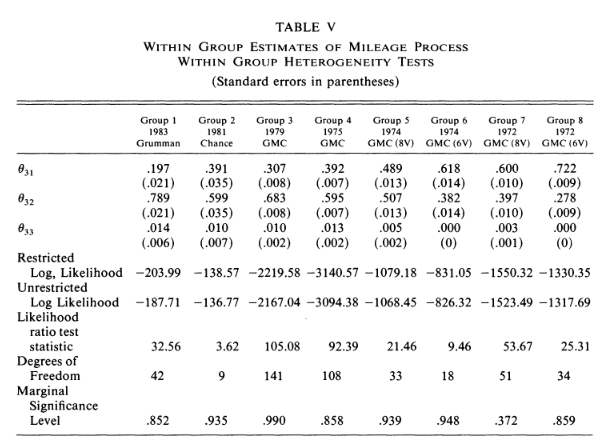
\includegraphics[scale =0.5]{t5.png}
\end{figure}
\end{center}
\end{frame}
\begin{frame}
\frametitle{Estimation-V}
\begin{center}
\begin{figure}[h!]
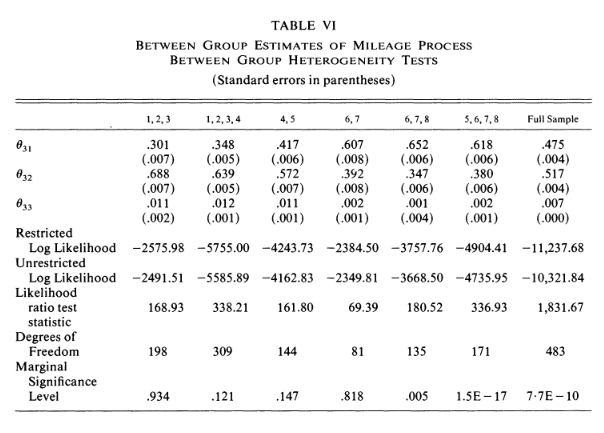
\includegraphics[scale =0.5]{t6.png}
\end{figure}
\end{center}
\end{frame}

\begin{frame}
\frametitle{Estimation-VI}
Given $\theta_3$, and using $\ell^2$ we can obtain estimates for $\beta$, $\theta_1$, and $RC$ ($RC=\overline{P}-\underline{P}$):
\[\ell^2(x_1,{...},x_T,i_1,{...}i,T)|\theta)=\prod_{t=1}^T P(i_t|x_t,\theta)\] where \[P(i|x,\theta)=\frac{\exp\{u(x,i,\theta_1)+\beta EV_\theta(x,i)\}}{\sum_{j\in C(x)}\exp\{u(x,j,\theta_1)+\beta EV_\theta(x,j)\}}\] with
\[EV_\theta(x,i)=\int_y\log\left\{ \sum_{j\in C(y)}\exp(u(y,j,\theta_1)+\beta EV_\theta (y,j))\right\}p(dy|x,i,\theta_3)\] and
\[u(x_t,i_t,\theta_1)+\varepsilon_t(i)=\left\{\begin{array}{lll} -RC-c(0,\theta_1)+\varepsilon_t(1)&if & i=1\\ -c(x_t,\theta_1)+\varepsilon_t(0)&if&i=0\end{array}\right.\]
\end{frame}


\begin{frame}
\frametitle{Estimation-VII}
\begin{itemize}
\item $\theta_1$ are the parameters of the cost function
\bigskip
\item Compare different (parsimonious) specifications 
\bigskip
\item Linear and square root forms do well
\end{itemize}
\end{frame}

\begin{frame}
\frametitle{Estimation-VIII}
\begin{center}
\begin{figure}[h!]
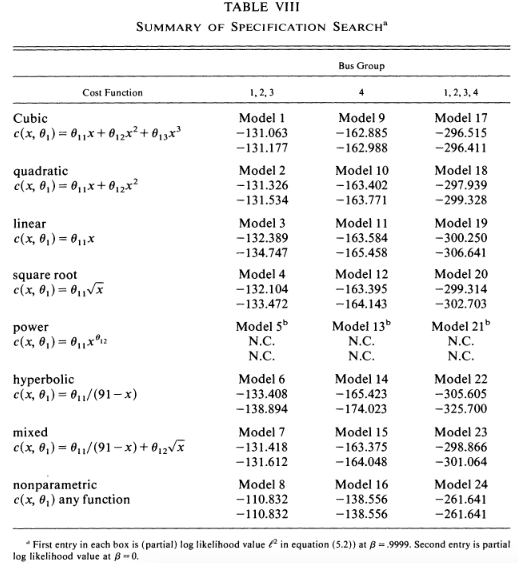
\includegraphics[scale =0.4]{t8.png}
\end{figure}
\end{center}
\end{frame}

\begin{frame}
\frametitle{Estimation-IX}
 
\begin{itemize}
\item Next look at ``myopic" replacement rule
\bigskip
\item replace only when operating costs $c(x_t,\theta_1)$ exceed current cost of replacement $RC+c(0,\theta_1)$
\bigskip
\item This model is rejected
\bigskip
\item $\beta = .999$ produces a statistically significantly better fit of the model to the data
\end{itemize}
\end{frame}

\begin{frame}
\frametitle{Estimation-VIII}
\begin{center}
\begin{figure}[h!]
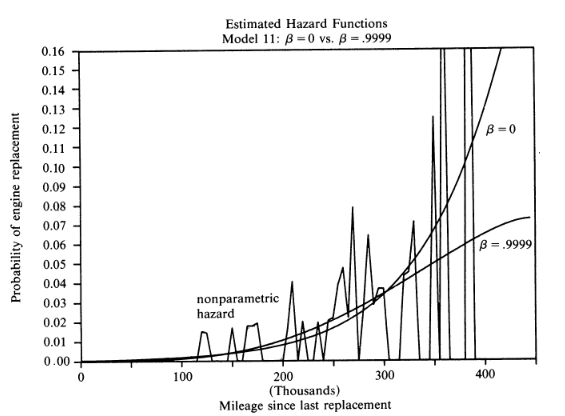
\includegraphics[scale =0.5]{f3.png}
\end{figure}
\end{center}
\end{frame}

\begin{frame}
\frametitle{Estimation-IX}
\begin{center}
\begin{figure}[h!]
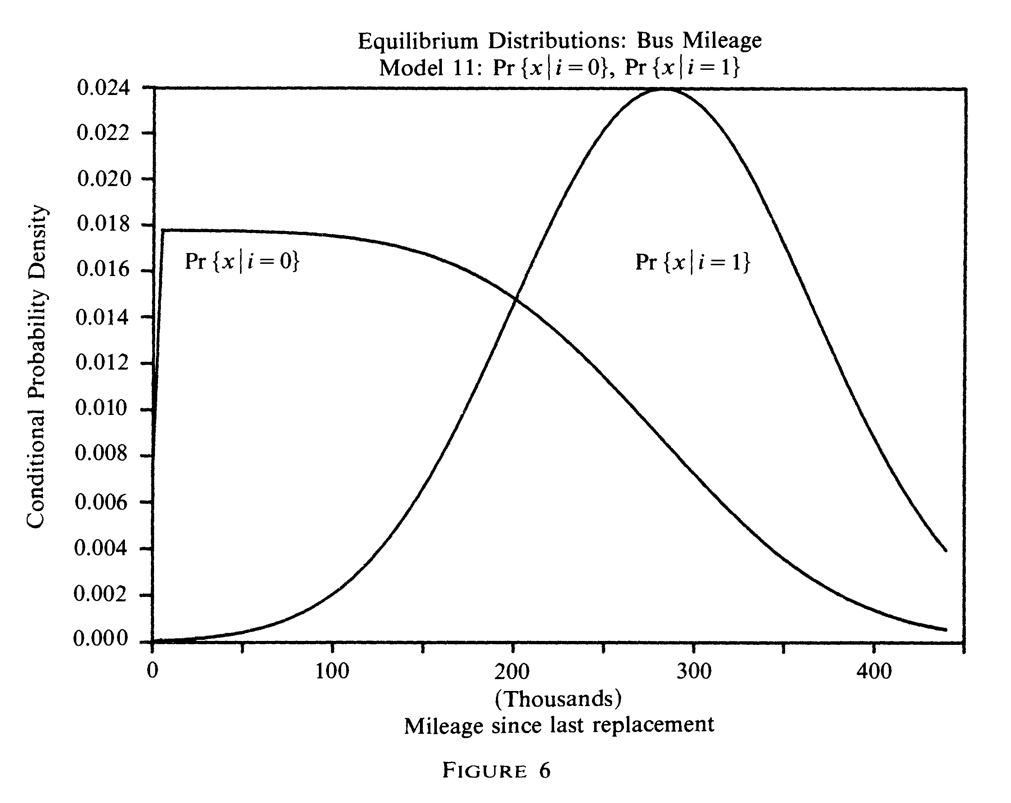
\includegraphics[scale =0.3]{Figure6.png}
\end{figure}
\end{center}
\end{frame}




\begin{frame}
\frametitle{Takeaways}
\begin{itemize}
\item<1-> So what?  Why not just do a logit?
\bigskip
\item<2-> Rust estimates Harold's problem at a micro level
\bigskip
\item<3-> Changes in interest rates, costs, etc. he can still deal with \emph{even if no variation in data!} 
\bigskip
\item<4-> Not myopic
\bigskip
\item<5-> Good example of indirectly inferring underlying parameters from agent behavior
\end{itemize}
\end{frame}

\begin{frame}
\frametitle{Counterfactuals}
\begin{center}
\begin{figure}[h!]
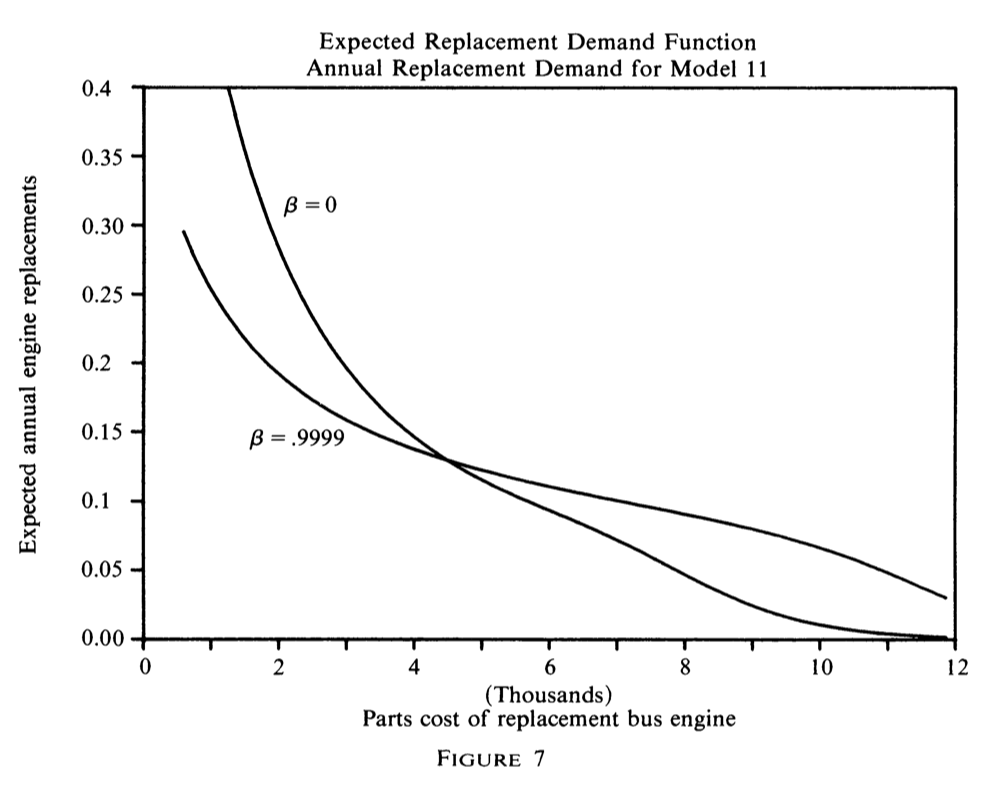
\includegraphics[scale =0.23]{Figure7.png}
\end{figure}
\end{center}
Because parts costs haven't changed, all \textbf{reduced form} estimates would be clustered around the intersection: unable to predict counterfactual reliably (not true of structural method)
\end{frame}

\begin{frame}
\frametitle{A better way?  MPEC}
\begin{itemize}
\item  Ordinarily, we have error function:  $g(\theta;X;V)$ and value function: $Vnew(\theta)=\max\left\{R+\beta Vold\right\}$.
\bigskip
\item Fixed point algorithm:
\begin{enumerate}
\item Given $\theta$, solve for $V$ (inner loop, many iterations)
\item Evaluate $g(\theta;X;V)$, find new $\theta$ to minimize $g$ (outer loop, needs precise inner loop)
\end{enumerate}
\item MPEC: put the inner loop in as a \emph{constraint}
$$\min_{\theta,V}\left\{g(\theta;X;V)\right\}\ \ \ s.t. Vnew(\theta)=\max\left\{R+\beta Vold\right\}$$
\item Idea: dont' need solve precisely for inner loop on bad $\theta$'s.
\item Much faster...3-800 times faster
\item Constraints could instead be equilibrium 
\begin{itemize}
\item BLP:  inner loop:  (shares(demand shocks($\theta$)), outer loop: choose $\theta$ to match moments
\end{itemize}
\end{itemize}
\end{frame}



\begin{frame}
\frametitle{Takeaways}
\begin{itemize}
\item Rust's method is a dynamic form of what we've been saying all semester
\bigskip
\item Most problems we write down have a natural fixed point in their estimation
\bigskip
\item Guess estimated parameters, can solve your model, simulate your model, calculate likelihoods from your model
\bigskip
\item With the feedback (errors, likelihood) can change parameters to minimize error, maximize likelihood, etc.
\bigskip
\item Rust gives a now-canonical example of how to do that in a dynamic discrete choice framework 
\end{itemize}
\end{frame}

\end{document}